\section{Materials and Methods}
\label{sec:methods}

The starting point for this project was a prior implementation~\cite{prior_impl} that
demonstrated the BLE communication pipeline, achieving 2\,kHz sampling on a single channel
via a CPU-polling loop. This approach had a fundamental limitation: the Nordic SoftDevice
preempts the application at every BLE connection event (every 10\,ms at the
empirically negotiated connection interval; the firmware-configured range is
7.5--10\,ms), preempting application code at the highest available interrupt priority levels; application
tasks cannot block it. For a peripheral connection event transmitting two to
three data packets, as required by the throughput demands of this system, the total
preemption time per connection event is typically approximately 400--500\,\textmu{}s (see
Appendix~\ref{app:softdevice_timing}) \cite[Table~36]{nordic_s132_sds_v72},
occurring every 10\,ms. In the prior
CPU-polling approach, this preemption directly interrupted the SPI acquisition loop,
causing missed samples. The reported 90\,kbps data rate furthermore reflects synthetic
test data rather than real acquisition: at 2\,kHz on a single 16-bit channel, the true
BLE throughput requirement is only 32\,kbps, while the reported 600\,kbps maximum was
demonstrated without real SPI data.

The present work addresses these limitations by replacing the CPU-polling loop with a
fully hardware-driven acquisition pipeline (PPI and EasyDMA), decoupling data acquisition
almost entirely from CPU availability. The design and implementation are described in
the subsections that follow.

\subsection{System Architecture Overview}

The wireless neural recording and stimulation system comprises four main components: (1) an Intan RHS2116 neural recording and stimulation chip interfaced via Serial Peripheral Interface (SPI, a wired synchronous serial protocol); (2) a Nordic nRF52832 microcontroller acting as the BLE peripheral, responsible for bidirectional communication with the Intan chip and wireless data transmission; (3) a second nRF52832 acting as the BLE central, which communicates wirelessly with the peripheral; and (4) a Python-based Graphical User Interface (GUI) running on a host computer for real-time visualization, control (including stimulation parameters), and data storage. 

\begin{figure}[h]
    \centering
    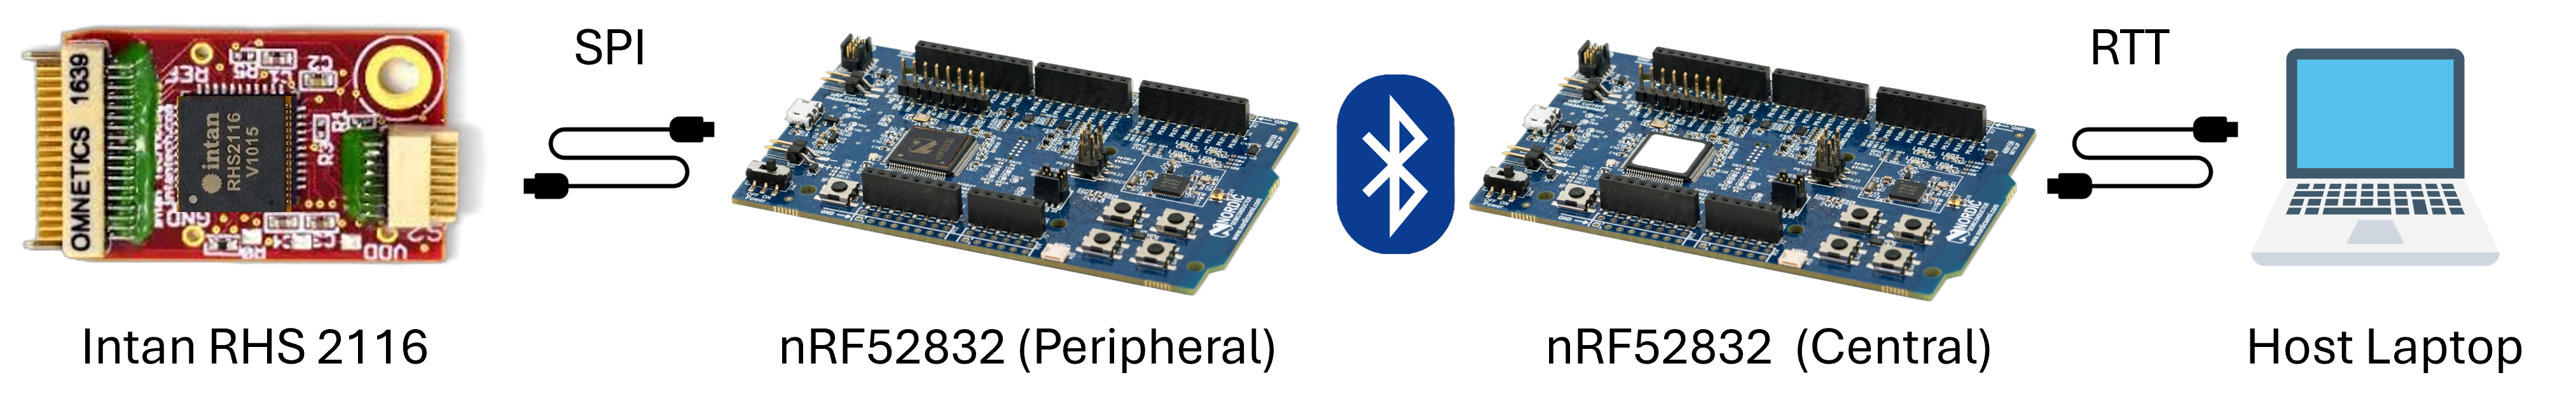
\includegraphics[width=\textwidth]{figures/system_overview.png}
    \caption{System architecture overview. The Intan RHS2116 neural 
    recording and stimulation chip communicates with the nRF52832 
    peripheral via SPI. The peripheral transmits data wirelessly to 
    the nRF52832 central via BLE, which forwards it to the host laptop 
    via RTT over USB. 
    \textit{Image sources: Intan RHS2116~\cite{intan_user_guide}; 
    nRF52832 Development Kit (DK)~\cite{nordic_dk_farnell};
    Bluetooth logo~\cite{bluetooth_svg_wikipedia}; 
    laptop icon~\cite{flaticon_laptop}.}}
    \label{fig:system_overview}
\end{figure}

Data flow proceeds as follows. In recording mode, the peripheral drives the Intan chip to continuously sample neural signals via SPI. Acquired samples are written directly to an active Direct Memory Access (DMA) buffer without CPU involvement, using the nRF52832's EasyDMA peripheral in list mode. When the active buffer approaches capacity (at approximately 80\% full), the CPU swaps the two DMA lists and resets the write pointer, allowing acquisition to continue uninterrupted into the previously inactive buffer. The data in the now-inactive buffer is then copied into a larger ring buffer, from which the CPU assembles structured packets for BLE transmission to the central. The central receives the packets and forwards them to the host computer via SEGGER Real-Time Transfer (RTT), a high-speed debug channel provided by the J-Link interface. The GUI parses the RTT data stream and renders voltage traces in real time.

The nRF52832 was chosen over comparable alternatives --- in particular the nRF52840,
which adds more RAM (256\,KB vs.\ 64\,KB), USB, and a higher maximum TX power --- on
the basis of size and power. The nRF52832 is available in a WLCSP49 package measuring
only $2.956 \times 3.226$\,mm, while the nRF52840's smallest package (WLCSP) measures
$3.544 \times 3.607$\,mm~\cite{nordic_nrf52840_ps} --- approximately 34\,\% larger by area.
On power, the nRF52832 draws approximately 5.3\,mA during BLE transmission at
0\,dBm with the DC/DC regulator enabled~\cite{nordic_nrf52832_pb}, compared to
approximately 6.4\,mA for the nRF52840 under the same
conditions~\cite{nordic_nrf52840_ps} --- a roughly 21\,\% increase.
Since the nRF52840 offers no functional advantage for this application --- neither
its additional RAM (256\,KB vs.\ 64\,KB), USB, nor its extended radio features
(Bluetooth Long Range, Direction Finding, Thread, Zigbee) are required --- the
nRF52832 is the clear choice: smaller, lower-power, and fully sufficient. The nRF52832 provides all required capabilities:
sufficient flash (512\,KB) and RAM (64\,KB) for the firmware, the PPI and EasyDMA
peripherals central to the acquisition pipeline, three independent SPIM and SPIS
instances, and BLE 5.0. No feature of the nRF52840 is required by the present design.

Firmware was initially developed on nRF52832 Development Kits (DKs); once stable,
it was also deployed to more compact modules, as described in
Section~\ref{sec:miniaturization}.


\begin{comment}
The wireless neural recording and stimulation system has four main hardware and software components: (1) an Intan RHS2116 neural recording/stimulation chip interfaced via Serial Peripheral Interface (SPI) communication, (2) a Nordic nRF52832 microcontroller acting as the Bluetooth Low Energy (BLE) peripheral responsible for bidirectional communication with the Intan for recording and stimulation mode and wireless transmission to a (3) second nRF52832 acting as the BLE central, which communicates to the peripheral and (4) a Python-based Graphical User Interface (GUI) running on a host computer for real-time visualization, control (including stimulation parameters), and data storage.

Data flow proceeds as follows: the peripheral handles the bidirectional communication with the Intan via SPI. In recording mode, the peripheral ensures that the Intan chip continuously samples neural signals. On the peripheral the data samples are written to the active easyDMA list. This described procedure is handled without CPU involvement. Once the active list is full, the second easyDMA list becomes the active list to which data is written to. After that switch, the data is copied from the inactive list into a larger ring buffer from which the data is assembled into a structured packet which is sent to the central using BLE. Contrary to the data acquisition, the packet creation and BLE functionality requires CPU involvement. The central receives the packets and forwards them  to the host computer via SEGGER Real-Time Transfer (RTT). The GUI parses the RTT data stream and renders the measured voltage traces in real-time.

For the firmware development, the nrf52832 development kits (DKs) were used as they provide integrated SEGGER J-Link interfaces, which enables direct RTT communication facilitating debugging to ensure efficient firmware development. 
\end{comment}
\subsection{Hardware Components and Specifications}

\subsubsection{Neural Recording/Stimulation Chip --- Intan RHS2116}
\label{sec:hardware_intan}

SPI (Serial Peripheral Interface) is a synchronous serial protocol in which one device,
the master (here the nRF52832), drives the clock (SCLK) and initiates every transaction,
while the other, the slave (here the Intan RHS2116), responds only when addressed.
Data flows simultaneously in both directions: MOSI (Master Out Slave In) carries the
command word from master to slave, while MISO (Master In Slave Out) returns the
response --- both clocked by SCLK. A chip-select (CS) line, asserted low by the master
for the duration of each transaction, identifies the intended slave and gates its
response.

The Intan RHS2116 is a 16-channel bidirectional neural interface chip combining
per-channel amplification, analog-to-digital conversion, and current-mode
stimulation.\footnote{Intan RHS2116 datasheet: \url{https://intantech.com/files/Intan_RHS2116_datasheet.pdf}~\cite{intan_rhs2116_datasheet}.}
Communication with the chip follows a 32-bit SPI transaction format: each transaction
consists of a 4-byte frame carrying a command type, register address, and 16-bit data
payload. The command set distinguishes between three primary operation classes:

\begin{itemize}
    \item \texttt{CONVERT(n)} commands that trigger an ADC conversion on channel~$n$
    and return the digitised result two SPI transactions later, owing to the chip's
    two-cycle conversion pipeline;
    \item \texttt{READ} commands that read a specified configuration register;
    \item \texttt{WRITE} commands that set a configuration register.
\end{itemize}

A subset of configuration registers --- including the stimulator enable registers (42,
44, 46, 48) and the stimulation amplitude registers (64--79, 96--111) --- are
\emph{triggered registers}: writes to these registers are staged in shadow storage and
only take effect when the U flag is asserted on any subsequent SPI transaction. This
allows multiple register changes to be prepared and applied atomically in a single
transaction, which is exploited in the stimulation pipeline to switch the current
polarity instantaneously between the cathodic and anodic phases
(Section~\ref{sec:stim_architecture}).

\paragraph{Amplifier Noise and Input Range.}
Each recording channel incorporates a high-gain amplifier with a band-pass
response and an input range of $\pm5$\,mV, providing sufficient headroom for
the signal amplitudes expected in neural recordings~\cite{intan_rhs2116_datasheet}.
The amplifier has a typical noise floor of 2.4\,\textmu{}V$_\text{rms}$~\cite{intan_rhs2116_datasheet}.
Following the standard peak-to-peak noise convention, the commonly used conversion
factor of $6.6\times$ the rms value---exceeded only 0.1\,\% of the
time~\cite[Chapter~1]{zumbahlen2011linear}\cite[Chapter~1]{jung2004op}---gives
a typical peak-to-peak noise floor of approximately
$6.6 \times 2.4 \approx 15.8$\,\textmu{}V$_\text{pp}$.
This characterises the practical sensitivity floor of the recording system
and is directly relevant to the noise characterisation presented in
Section~\ref{sec:results_noise}.

\paragraph{Chip Initialisation.}
The initialisation sequence follows the example procedure in the RHS2116
datasheet~\cite{intan_rhs2116_datasheet} (pp.~44--45). The lower amplifier bandwidth is
fixed at $f_L = 5$\,Hz, appropriate for LFP recording. The only notable deviation is
that the upper bandwidth~$f_H$ is not configured during initialisation; it is instead
written at every acquisition start via \texttt{rhs\_set\_bandwidth()}, enabling the
upper bandwidth to be adjusted from the GUI based on the configured sampling rate
(see Section~\ref{sec:ppi_acquisition}).

\paragraph{Recording Configuration and Channel Selection.}
For continuous multi-channel recording, the chip is driven with a
\texttt{CONVERT(63)} command --- a special auto-sequencing instruction that causes the
RHS2116 to multiplex through all 16 channels in order, advancing to the next channel
on each successive SPI transaction~\cite{intan_rhs2116_datasheet}. This allows the
peripheral to send a single fixed 32-bit command word on every transaction, with the
chip handling channel cycling internally. This property is the key enabler of the
hardware-driven acquisition architecture: because the PPI subsystem triggers SPI
transactions at a fixed rate independent of CPU state, requiring only a single repeated
command allows the firmware to delegate the entire transaction sequence to hardware
without tracking channel state in software. Because the same word repeats indefinitely,
no SPI TX command buffer is required: the nRF52832 drives MOSI with a single fixed
32-bit word that DMA repeats automatically. Without \texttt{CONVERT(63)}'s
auto-sequencing, a TX command buffer of one word per DMA transfer would be needed ---
equal in size to the RX sample buffer --- and firmware would additionally need to
track the current channel offset across DMA list switches to re-phase the cyclic
\texttt{CONVERT(0..15)} sequence correctly, a non-trivial synchronisation concern
absent from the present design. Only samples from logically selected channels (configured via a
16-bit bitmask from the GUI) are forwarded to the receive buffer
(Section~\ref{sec:ppi_acquisition}); the remaining samples are discarded in firmware.
Because \texttt{CONVERT(63)} always cycles all 16 physical channels regardless of how
many are selected, the per-channel sampling rate is always the total SPI transaction
rate divided by 16 in this mode. For example, recording 8 channels at 4\,kHz per
channel still requires $16 \times 4\,\text{kHz} = 64\,\text{kHz}$ total SPI
transactions per second --- twice as many as for 16 channels at 2\,kHz each. The
total SPI transaction rate is subject to a hardware ceiling (quantified in
Section~\ref{sec:ppi_acquisition}): the timer period must be long enough for each
32-bit transaction to complete before the next one fires. For higher per-channel rates
with fewer active channels, a dedicated single-channel mode issues
\texttt{CONVERT($k$)} directly, bypassing the 16-cycle overhead: recording one channel
at 32\,kHz requires only 32\,kHz SPI transactions per second, whereas
\texttt{CONVERT(63)} would demand $16 \times 32\,\text{kHz} = 512\,\text{kHz}$ ---
not achievable in practice. The
achievable per-channel rates for each configuration and the resulting BLE throughput
are summarised in Section~\ref{sec:results}.

\paragraph{Power Supply.}
The \texttt{VSTIM} power supply pins must never be left floating, as this causes
excessive power dissipation~\cite[p.~24]{intan_rhs2116_datasheet}. When stimulation is not in
use, \texttt{VSTIM+} can be tied to \texttt{VDD} and \texttt{VSTIM-} to ground. When
stimulation is active, a bipolar supply is required: \texttt{VSTIM+} must be in the
range $+3.3$\,V to $+10.7$\,V with respect to ground, \texttt{VSTIM-} in the range
$-3.3$\,V to $-10.7$\,V, and the total supply (\texttt{VSTIM+} $-$ \texttt{VSTIM-})
must not exceed 14\,V~\cite{intan_rhs2116_datasheet}. In the bench-top test
configuration, $\pm5$\,V was provided by a signal generator with a common ground
reference, giving a total of 10\,V and remaining within the 14\,V limit with comfortable
margin.

To provide accessible connections to the RHS2116 pin header during bench-top testing,
the chip was mounted on a small carrier board (Figure~\ref{fig:intan_board}).
The pin assignment of the 40-pin connector, derived from the official Intan RHS 32-channel
headstage pinout,\footnote{\url{https://intantech.com/RHS_headstages.html?tabSelect=RHS32ch}}
is shown in Figure~\ref{fig:connector_pinout}.

\begin{figure}[h]
    \centering
    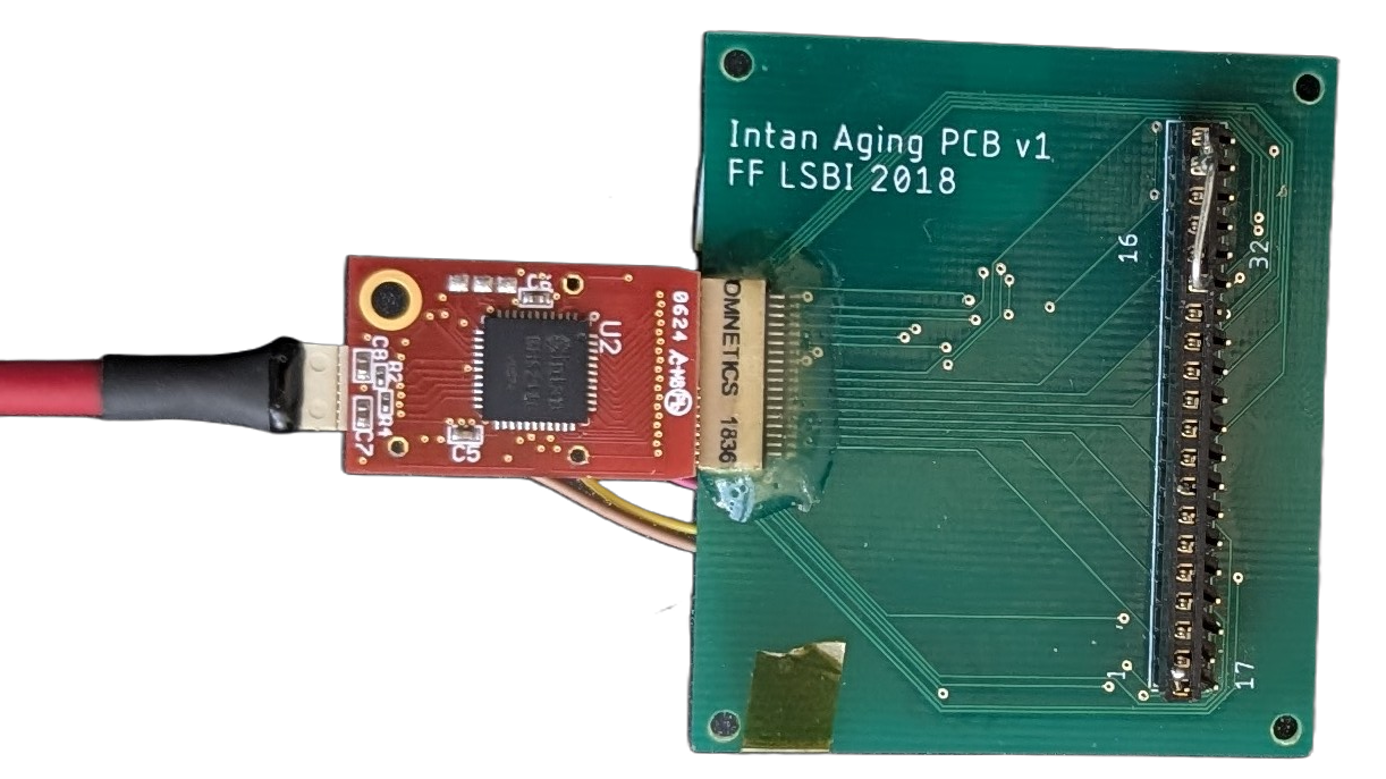
\includegraphics[width=0.45\textwidth]{figures/intan_green_board_horizontal.png}
    \caption{Intan RHS2116 chip (black die) mounted on its green carrier board,
    providing accessible pin headers for bench-top SPI connections during development.}
    \label{fig:intan_board}
\end{figure}

\begin{figure}[htbp]
\centering
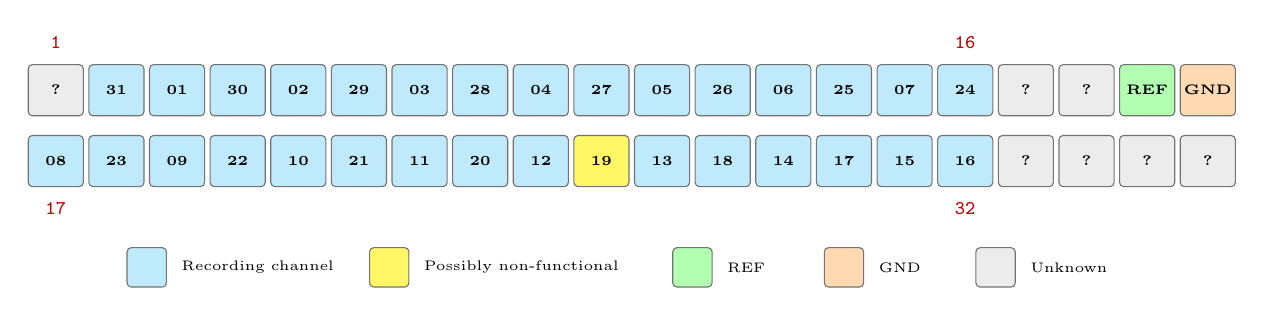
\begin{tikzpicture}[
  pin/.style={
    draw=black!55, rounded corners=1.5pt,
    minimum width=7mm, minimum height=6.5mm,
    font=\tiny\bfseries, inner sep=0pt, align=center
  }
]
\colorlet{Cch}{cyan!25}
\colorlet{Cnw}{yellow!60}
\colorlet{Cref}{green!30}
\colorlet{Cgnd}{orange!30}
\colorlet{Cunk}{gray!15}
\def\dx{0.77cm}
\def\topy{0.9cm}
\def\boty{0cm}
%% TOP ROW
\node[pin,fill=Cunk] (T1)  at ( 0*\dx,\topy) {?};
\node[pin,fill=Cch]  (T2)  at ( 1*\dx,\topy) {31};
\node[pin,fill=Cch]  (T3)  at ( 2*\dx,\topy) {01};
\node[pin,fill=Cch]  (T4)  at ( 3*\dx,\topy) {30};
\node[pin,fill=Cch]  (T5)  at ( 4*\dx,\topy) {02};
\node[pin,fill=Cch]  (T6)  at ( 5*\dx,\topy) {29};
\node[pin,fill=Cch]  (T7)  at ( 6*\dx,\topy) {03};
\node[pin,fill=Cch]  (T8)  at ( 7*\dx,\topy) {28};
\node[pin,fill=Cch]  (T9)  at ( 8*\dx,\topy) {04};
\node[pin,fill=Cch]  (T10) at ( 9*\dx,\topy) {27};
\node[pin,fill=Cch]  (T11) at (10*\dx,\topy) {05};
\node[pin,fill=Cch]  (T12) at (11*\dx,\topy) {26};
\node[pin,fill=Cch]  (T13) at (12*\dx,\topy) {06};
\node[pin,fill=Cch]  (T14) at (13*\dx,\topy) {25};
\node[pin,fill=Cch]  (T15) at (14*\dx,\topy) {07};
\node[pin,fill=Cch]  (T16) at (15*\dx,\topy) {24};
\node[pin,fill=Cunk] (T17) at (16*\dx,\topy) {?};
\node[pin,fill=Cunk] (T18) at (17*\dx,\topy) {?};
\node[pin,fill=Cref] (T19) at (18*\dx,\topy) {REF};
\node[pin,fill=Cgnd] (T20) at (19*\dx,\topy) {GND};
%% BOTTOM ROW
\node[pin,fill=Cch]  (B1)  at ( 0*\dx,\boty) {08};
\node[pin,fill=Cch]  (B2)  at ( 1*\dx,\boty) {23};
\node[pin,fill=Cch]  (B3)  at ( 2*\dx,\boty) {09};
\node[pin,fill=Cch]  (B4)  at ( 3*\dx,\boty) {22};
\node[pin,fill=Cch]  (B5)  at ( 4*\dx,\boty) {10};
\node[pin,fill=Cch]  (B6)  at ( 5*\dx,\boty) {21};
\node[pin,fill=Cch]  (B7)  at ( 6*\dx,\boty) {11};
\node[pin,fill=Cch]  (B8)  at ( 7*\dx,\boty) {20};
\node[pin,fill=Cch]  (B9)  at ( 8*\dx,\boty) {12};
\node[pin,fill=Cnw]  (B10) at ( 9*\dx,\boty) {19};
\node[pin,fill=Cch]  (B11) at (10*\dx,\boty) {13};
\node[pin,fill=Cch]  (B12) at (11*\dx,\boty) {18};
\node[pin,fill=Cch]  (B13) at (12*\dx,\boty) {14};
\node[pin,fill=Cch]  (B14) at (13*\dx,\boty) {17};
\node[pin,fill=Cch]  (B15) at (14*\dx,\boty) {15};
\node[pin,fill=Cch]  (B16) at (15*\dx,\boty) {16};
\node[pin,fill=Cunk] (B17) at (16*\dx,\boty) {?};
\node[pin,fill=Cunk] (B18) at (17*\dx,\boty) {?};
\node[pin,fill=Cunk] (B19) at (18*\dx,\boty) {?};
\node[pin,fill=Cunk] (B20) at (19*\dx,\boty) {?};
%% BOARD ORIENTATION MARKERS
\node[font=\scriptsize\bfseries, red!75!black, above=2pt] at (T1.north)  {\texttt{1}};
\node[font=\scriptsize\bfseries, red!75!black, above=2pt] at (T16.north) {\texttt{16}};
\node[font=\scriptsize\bfseries, red!75!black, below=2pt] at (B1.south)  {\texttt{17}};
\node[font=\scriptsize\bfseries, red!75!black, below=2pt] at (B16.south) {\texttt{32}};
%% LEGEND
\node[pin,fill=Cch,  minimum size=5mm] at ( 1.5*\dx,-1.35cm) {};
\node[anchor=west, font=\tiny] at ( 1.5*\dx+0.32cm,-1.35cm) {Recording channel};
\node[pin,fill=Cnw,  minimum size=5mm] at ( 5.5*\dx,-1.35cm) {};
\node[anchor=west, font=\tiny] at ( 5.5*\dx+0.32cm,-1.35cm) {Possibly non-functional};
\node[pin,fill=Cref, minimum size=5mm] at (10.5*\dx,-1.35cm) {};
\node[anchor=west, font=\tiny] at (10.5*\dx+0.32cm,-1.35cm) {REF};
\node[pin,fill=Cgnd, minimum size=5mm] at (13.0*\dx,-1.35cm) {};
\node[anchor=west, font=\tiny] at (13.0*\dx+0.32cm,-1.35cm) {GND};
\node[pin,fill=Cunk, minimum size=5mm] at (15.5*\dx,-1.35cm) {};
\node[anchor=west, font=\tiny] at (15.5*\dx+0.32cm,-1.35cm) {Unknown};
\end{tikzpicture}
\caption{Pin assignment of the Intan RHS2116 carrier board connector (40 pins,
2 rows $\times$ 20 columns, shown horizontally). Numbers inside pin boxes are
Intan channel indices. Red numbers (\texttt{1}, \texttt{16}, \texttt{17},
\texttt{32}) are orientation markers printed on the physical board.
Channel~19 (yellow) was intermittently non-functional during testing.
Grey pins were not characterised. The carrier board is shown in
Figure~\ref{fig:intan_board}.}
\label{fig:connector_pinout}
\end{figure}

When this
assembly was placed inside the wireless power transfer transmitter coil field, significant
electromagnetic interference was observed on the recorded signals; this is discussed
further in Section~\ref{sec:results_noise}. % \TODO{adjust section ref}
Power consumption of the nRF52832 module alone was measured in the 16-channel,
2\,kHz per channel configuration. Power consumption of the combined nRF52832 and
Intan RHS2116 system was characterised across a range of channel count and
sampling rate configurations; results are reported in
Section~\ref{sec:results_power}.

\subsubsection{Microcontroller --- Nordic nRF52832}
The Nordic nRF52832 is a 32-bit ARM Cortex-M4F system-on-chip (SoC) with an
integrated 2.4\,GHz radio supporting Bluetooth~5.3~\cite{nordic_nrf52832_pb}.
It includes 512\,kB of flash memory, 64\,kB of RAM, multiple hardware timers,
a Programmable Peripheral Interconnect (PPI) crossbar enabling direct
peripheral-to-peripheral event routing without CPU involvement, and an
EasyDMA-capable SPI Master (SPIM) peripheral.

Bluetooth Low Energy (BLE) is a short-range wireless protocol designed for
sensor applications where the radio is active only during brief, scheduled
transmission bursts, keeping average power consumption low~\cite{tosi2017performance}.
Connections follow an asymmetric peripheral--central model: the peripheral
(sensor node) proactively sends data to the central at each connection interval.
In this system the central role is filled by a dedicated second nRF52832 module
rather than the host laptop directly, for two reasons. First, the central module
can be positioned in close physical proximity to the peripheral --- relevant for
animal experiments where it may be convenient to keep the laptop at a distance. Second, forwarding
data from the central to the laptop via J-Link RTT is fully OS-independent, whereas
programming a laptop's integrated BLE hardware at the required low level may not be
feasible or portable across different operating systems and hardware configurations.

The firmware was developed using the Nordic nRF5 SDK with the S132
SoftDevice~\cite{nordic_s132_sds_v72}, Nordic's pre-compiled, protocol-certified
BLE stack. The SoftDevice manages all BLE radio operations, connection
maintenance, and timing --- tasks that would otherwise require significant
implementation effort and re-certification. In doing so it occupies a reserved
region of flash and RAM, and operates at the highest available interrupt priority
levels (0, 1, and~4), preempting application code at every scheduled BLE radio
event (every connection interval of approximately 10\,ms). The implications of
this preemption for hardware-driven acquisition timing are discussed in
Appendix~\ref{app:softdevice_timing}. Timer~0 is reserved by the SoftDevice and unavailable to application code.

During firmware development, both the peripheral and central were operated as
nRF52832 Development Kits (DKs). The DK's integrated SEGGER J-Link debugger
enables both real-time debugging via RTT and direct firmware flashing without
additional hardware --- in contrast to standalone modules, which require an
external J-Link connection as described in Appendix~\ref{app:flash_ndk}. The
peripheral was subsequently miniaturized through a progression of smaller
modules, as described in Section~\ref{sec:miniaturization}. Software requirements for running the system and
for firmware development are listed in Appendices~\ref{app:software_run}
and~\ref{app:software_dev} respectively.

\subsubsection{Hardware Miniaturization}
\label{sec:miniaturization}

Following successful firmware validation on the nRF52832 DK, the peripheral
was progressively miniaturized toward a form factor compatible with implantable
use, with end-to-end functionality verified at each stage before proceeding
to the next. Figure~\ref{fig:miniaturization} shows the three stages of this
progression. The first step replaced the DK with a SparkFun nRF52832 Breakout
board~\cite{sparkfun_nrf52832}, which provides accessible pin headers and a USB
port for power supply (USB does not support firmware flashing or debugging on
this board; see Appendix~\ref{app:flash_ndk} for the flashing procedure), while being significantly more
compact. The subsequent two stages used custom nRF52832 modules designed by
Ivan Furfaro, stripped down to only the components required for
operation and firmware flashing: two LEDs and the
necessary programming pins, with no buttons or other peripherals. The final
step further reduces the nRF52832 chip itself from the QFN48
(6$\times$6\,mm, 48 pins~\cite[p.~544]{nordic_nrf52832_ps}) to the WLCSP49
(2.956$\times$3.226\,mm, 49 solder balls~\cite[p.~545]{nordic_nrf52832_ps})
package, achieving the most compact form factor. The miniaturized
peripheral was validated end-to-end under wireless power transfer conditions,
as described in Section~\ref{sec:results_noise}.

\begin{figure}[h]
    \centering
    \begin{subfigure}[b]{0.22\textwidth}
        \centering
        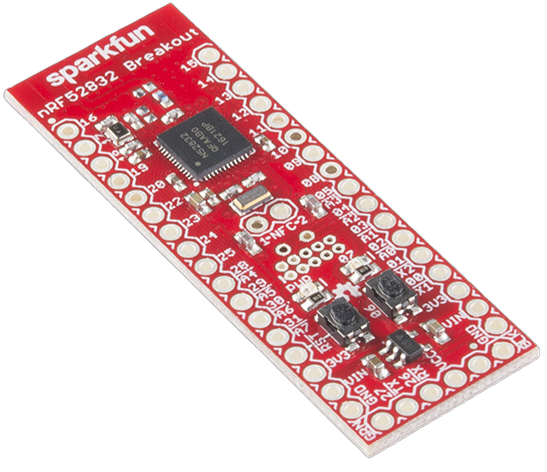
\includegraphics[width=\textwidth]{figures/nrf_sparkfun.png}
        \caption{SparkFun nRF52832 Breakout~\cite{sparkfun_nrf52832}}
    \end{subfigure}
    \hfill
    \begin{subfigure}[b]{0.22\textwidth}
        \centering
        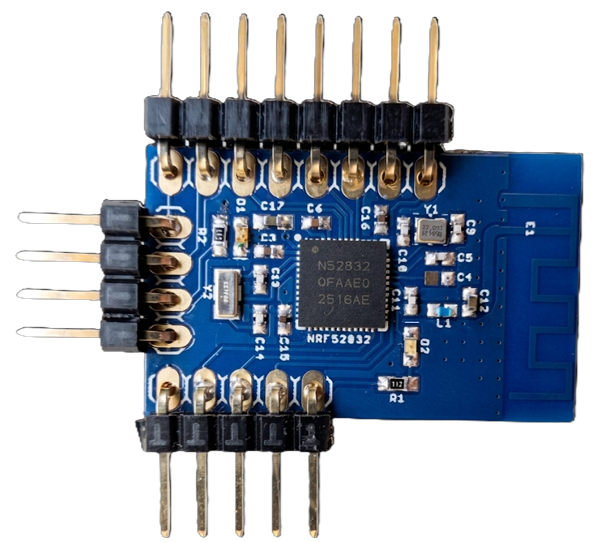
\includegraphics[width=\textwidth]{figures/nrf_peripheral_qfn_blue.png}
        \caption{Custom module, QFN48 package}
    \end{subfigure}
    \hfill
    \begin{subfigure}[b]{0.22\textwidth}
        \centering
        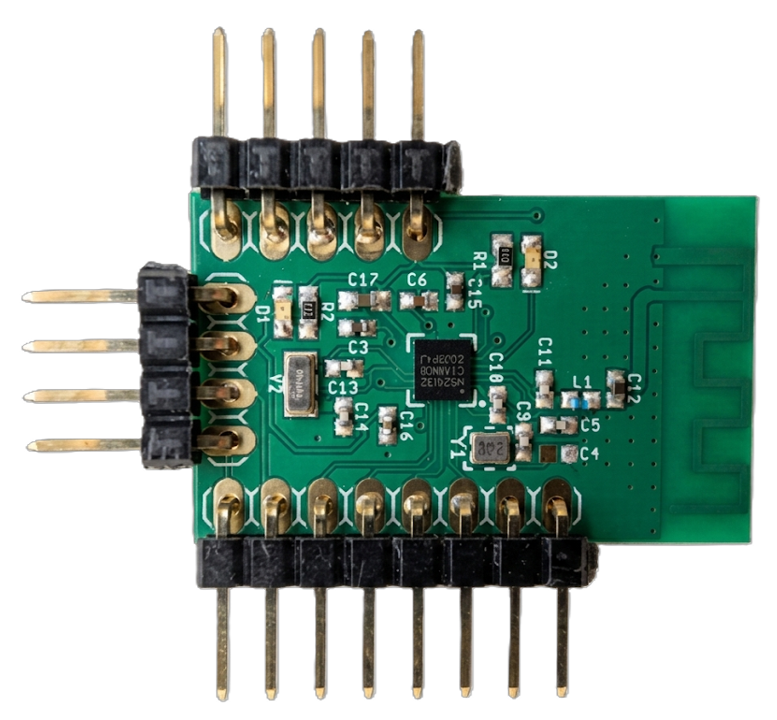
\includegraphics[width=\textwidth]{figures/nrf_peripheral_wlcsp_green.png}
        \caption{Custom module, WLCSP49 package}
    \end{subfigure}
    \hfill
    \begin{subfigure}[b]{0.22\textwidth}
        \centering
        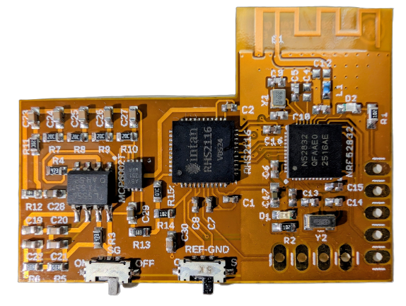
\includegraphics[width=\textwidth]{figures/nrf_intan_oscillator.png}
        \caption{Flex PCB co-integrating nRF52832 and Intan RHS2116}
    \end{subfigure}
    \caption{Miniaturization progression toward an integrated neural recording module.
    (a) SparkFun nRF52832 Breakout board, used for initial development (50$\times$16\,mm).
    (b) Custom QFN48 nRF52832 module (29$\times$17\,mm).
    (c) Custom WLCSP49 nRF52832 module, most compact standalone module (29$\times$17\,mm).
    (a)--(c) run identical firmware and each interface with the Intan RHS2116 via an
    external carrier board (see Figure~\ref{fig:wiring_connector}).
    (d) Prototype flex PCB co-integrating the nRF52832 and Intan RHS2116 on the same
    substrate (non-rectangular outline, bounding box 39$\times$29\,mm), with an
    on-board square-wave oscillator switchable to Intan input pin~0, intended for
    calibration signal injection in the wireless power transfer field
    (see Section~\ref{sec:results_noise}).}
    \label{fig:miniaturization}
\end{figure}

\begin{figure}[h]
    \centering
    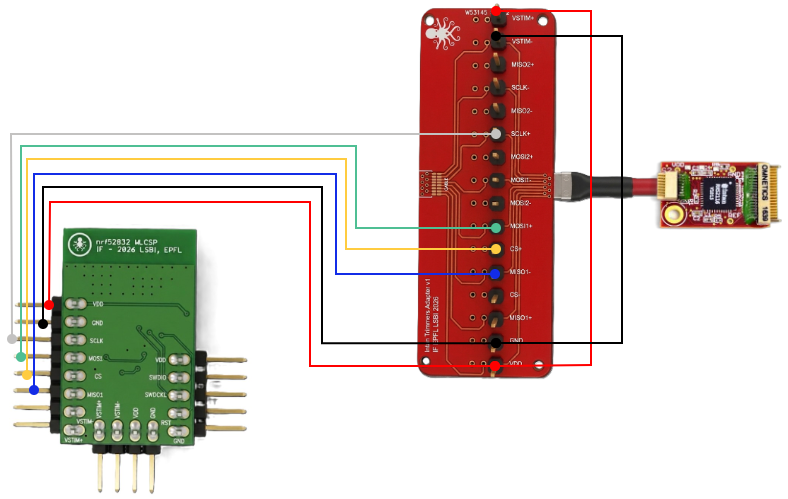
\includegraphics[width=0.9\textwidth]{figures/wiring_intan_wlcsp_connector_board.png}
    \caption{Connection setup for the standalone nRF52832 modules. An intermediate
    carrier board routes SPI signals and power between the nRF52832 module pin header
    and the standard Intan headstage connector. The QFN48 module is shown; the
    SparkFun breakout and WLCSP49 modules use the same carrier board with equivalent
    connections.}
    \label{fig:wiring_connector}
\end{figure}

Firmware flashing of the standalone modules and the required software installation are
described in Appendices~\ref{app:flash_ndk} and~\ref{app:software_dev} respectively.

\paragraph{Wireless Power Transfer Noise Characterisation.}
The miniaturized peripheral was operated under wireless power by placing the receive
coil of the WPT system (developed by Marta Vasconcelos within the lab)
in the field of the transmitter coil, with the remainder of the system --- the
nRF52832 module, the Intan RHS2116 on its green carrier board, and the connecting
cables --- positioned at a distance of approximately 30--50\,cm from the transmitter
coil. Under this arrangement the system recorded and transmitted neural data
successfully, confirming end-to-end wireless operation
(see Section~\ref{sec:results_noise}).

To characterise signal quality, a sinusoidal test signal from a function
generator (NTi Minirator MR2/MR-PRO~\cite{nti_minirator_mr2} or Keysight
33500B Series~\cite{keysight_33500b}) was injected into one recording channel via the
carrier board connector (one terminal to the electrode input, the other to
GND/REF). Throughout bench testing the RHS2116 REF input was shorted to GND:
without a tissue reference electrode present, this provides a stable 0\,V
reference for the on-chip differential amplifiers.
With the green carrier board and the function generator cables far from
the transmitter coil, the recorded sine wave was clean. As the assembly was moved
progressively closer to the transmitter, the signal became increasingly corrupted
by interference; the degree of corruption also depended on how close the function
generator cables themselves were to the transmitter coil. This distance-dependent
behaviour, and its sensitivity to external cable routing, suggested that the
long signal cables were acting as pickup antennas or forming inductive loops in
the transmitter field --- rather than the interference originating inside the chip
itself.
Figure~\ref{fig:wtp_setup} shows the Intan RHS2116 on its carrier board with the
receive coil positioned inside the transmitter coil.

To quantify electromagnetic interference pickup systematically, a recording channel
was shorted to GND as close to the GND supply pin as possible. Channel~7 was
selected as it is the nearest accessible recording channel to the GND and REF pins
on the carrier board connector (Figure~\ref{fig:connector_pinout}). The headstage
used here carries two RHS2116 chips (channels~1--16 on one chip, channels~17--32 on
the other); only one chip was interfaced via SPI, making channels~1--16 the
accessible set. A GND-shorted channel ideally produces only the amplifier's intrinsic
noise floor; any signal substantially above this floor represents interference pickup. Measurements were made at three positions relative to
the transmitter coil: 30\,cm (reference baseline), 4\,cm from the coil edge, and
fully inside the coil, in all cases with the carrier board and its wiring in place.
Results from these measurements are presented in Section~\ref{sec:results_noise}.

The carrier-board measurements inside the WPT field revealed severe
saturation-level interference (Section~\ref{sec:results_noise}). To assess how much
of this originates from the board wiring rather than from the chip or the WPT field
acting directly on the silicon, a second measurement was made with channel~1 shorted
directly on the Intan RHS2116 die, bypassing the carrier board connector entirely.

Finally, the prototype flex PCB (Figure~\ref{fig:miniaturization}d), which
integrates an on-board square-wave oscillator switchable to Intan input pin~0, was
intended to provide a defined test signal inside the WPT field without any external
signal wiring. Its use would allow verification that the signal path is functional
in a co-integrated configuration.

\begin{figure}[h]
    \centering
    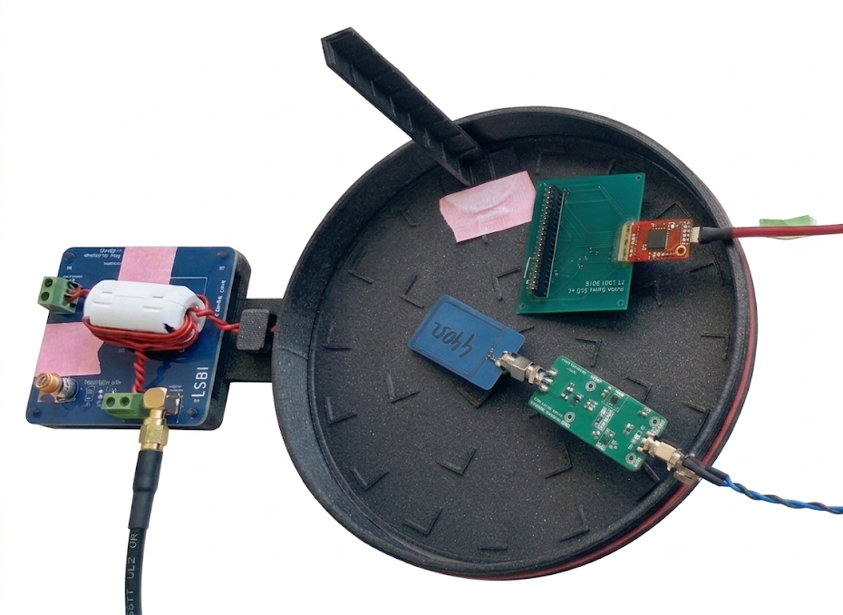
\includegraphics[width=0.6\textwidth]{figures/wtp_coil_rx_coil_intan.png}
    \caption{Experimental setup for wireless power transfer validation. The Intan
    RHS2116 on its carrier board, with the WPT receive coil attached, is shown
    inside the transmitter coil field.}
    \label{fig:wtp_setup}
\end{figure}


\subsection{Peripheral Firmware --- Recording Pipeline}
\subsubsection{PPI-Driven SPI Acquisition}
\label{sec:ppi_acquisition}

To decouple data acquisition from CPU availability, the nRF52832's Programmable
Peripheral Interconnect (PPI) subsystem is used to connect hardware peripherals
directly, without CPU involvement in each SPI transaction.\footnote{All firmware source code is available at:
\url{https://github.com/Simonseyfert/ble_spi_intan} (private repository;
access available upon request at \href{mailto:simon.seyfert@epfl.ch}{simon.seyfert@epfl.ch}
or \href{mailto:simon.seyfert@tum.de}{simon.seyfert@tum.de}).}
The SPI master peripheral (SPIM0) is operated in EasyDMA list mode, where received
bytes are written directly to a memory buffer by the DMA engine --- without any
CPU involvement.

Four PPI channels coordinate all hardware-driven acquisition events --- SPI
triggering, chip-select control, and transaction counting --- entirely without CPU
involvement, and are enabled at the start of each acquisition, as summarised in
Table~\ref{tab:ppi_channels}.

\begin{table}[htbp]
\centering
\caption{PPI channel configuration for hardware-driven SPI acquisition.}
\label{tab:ppi_channels}
\begin{tabular}{lll}
\toprule
\textbf{Event Source}    & \textbf{Task Destination}  & \textbf{Purpose} \\
\midrule
Timer1 \texttt{COMPARE0} & \texttt{SPIM START}        & Trigger SPI transaction \\
Timer1 \texttt{COMPARE0} & \texttt{GPIOTE OUT[0]}     & Assert CS low (toggle) \\
\texttt{SPIM END}        & \texttt{GPIOTE OUT[0]}     & Release CS high (toggle) \\
\texttt{SPIM END}        & Timer2 \texttt{COUNT}      & Increment transaction counter \\
\bottomrule
\end{tabular}
\end{table}

GPIOTE (General-Purpose I/O Tasks and Events) is the nRF52832's hardware module
that allows physical output pins to be driven high or low in response to internal
hardware events --- such as a timer reaching a threshold or an SPI transaction
completing --- without the CPU needing to execute any code.
GPIOTE channel~0 is configured in toggle mode, starting high, to drive the CS line.
Both CS events are routed to the same \texttt{GPIOTE OUT[0]} toggle output: the
Timer1 \texttt{COMPARE0} event pulls CS low at the start of each transaction, and
the \texttt{SPIM END} event releases it high at completion.

Timer1 runs continuously, resetting on each compare match. Its period is set at the
start of each acquisition to produce the required inter-transaction interval. The
nRF52832 timers run at 16\,MHz, giving a resolution of 62.5\,ns per tick.
In multi-channel mode, \texttt{CONVERT(63)} cycles all 16 channels at a total SPI
rate of $16f$ transactions per second, where $f$ is the per-channel sampling rate.
A convenient coincidence simplifies the arithmetic: the factor of 16 from cycling
all channels and the 16\,MHz clock rate (16\,ticks/\textmu s) cancel exactly,
yielding:
\begin{equation}
    T_\text{ticks} = \mathrm{round}\!\left(\frac{1\,000\,000}{f}\right)
    \label{eq:timer_period}
\end{equation}
where $f$ is in Hz and $T_\text{ticks}$ is the timer period in 16\,MHz ticks.
For example, at $f = 2$\,kHz per channel: $T_\text{ticks} = 500$\,ticks\,$= 31.25$\,\textmu s,
giving a total SPI rate of 32\,kHz. In single-channel mode, the factor of 16 does
not cancel, giving $T_\text{ticks} = \mathrm{round}(16\,000\,000/f)$ ticks.

Timer2 counts completed SPI transactions via the PPI link from each
\texttt{SPIM END} event. When it reaches 819 (80\,\% of the 1024-slot DMA buffer
capacity), it fires an interrupt that swaps the two DMA buffers, allowing
acquisition to continue uninterrupted while the CPU processes the completed data;
this is described in detail in the following section.

\subsubsection{Double-Buffering and Ring Buffer}

Two DMA buffers, \texttt{dma\_buffer\_a} and \texttt{dma\_buffer\_b}, each
\texttt{DMA\_BUF\_BYTES} $= 4096$\,bytes (\texttt{DMA\_BUF\_SAMPLES} $= 1024$
samples $\times$ 4\,bytes/sample), are maintained as a double-buffer pair. Each
buffer is aligned to its own size in memory (\texttt{\_\_attribute\_\_((aligned(DMA\_BUF\_BYTES)))}).
The nRF52832 EasyDMA does not strictly require aligned buffers, but the alignment
is applied as a precautionary measure to prevent potential data corruption from
memory boundary crossing in EasyDMA list mode. The invariant is
strict: the PPI and EasyDMA pipeline writes exclusively to the active buffer, while
the CPU reads exclusively from the inactive buffer (copying samples to the ring
buffer). No buffer is ever accessed by both sides simultaneously.

When Timer2 reaches a threshold of 819 transactions (80\,\% of
\texttt{DMA\_BUF\_SAMPLES}), the \texttt{timer2\_count\_handler} ISR fires. The
buffer swap is performed inside a SoftDevice critical section
(\texttt{sd\_nvic\_critical\_region\_enter}/\texttt{exit}). A critical section
disables all maskable CPU interrupts --- including the SoftDevice's BLE radio and
protocol ISRs --- so that nothing can preempt the code between \texttt{enter} and
\texttt{exit}. This atomicity is essential: the protected sequence stops Timer1
(halting data acquisition), updates the DMA write pointer to the new buffer, and
resumes Timer1 (restarting acquisition). Without this protection, an interrupt
occurring after Timer1 is stopped but before it is restarted would extend the
acquisition gap beyond ${\approx}250$\,ns, causing sample loss during that delay:

\begin{lstlisting}[language=C]
sd_nvic_critical_region_enter(&is_nested);
nrf_drv_timer_pause(&timer1);
uint32_t samples_done =
    (NRF_SPIM0->RXD.PTR - (uint32_t)active_dma_buffer) / 4;
uint8_t *temp        = active_dma_buffer;
active_dma_buffer    = inactive_dma_buffer;
inactive_dma_buffer  = temp;
NRF_SPIM0->RXD.PTR   = (uint32_t)active_dma_buffer;
nrf_drv_timer_clear(&timer2);
if (!stop_requested) nrf_drv_timer_resume(&timer1);
sd_nvic_critical_region_exit(is_nested);
\end{lstlisting}

The completed sample count is read directly from the EasyDMA hardware write
pointer rather than assumed to be exactly 819. This is necessary because the
timer2 ISR may have been delayed: when Timer2 reaches 819 the ISR should fire,
but if the SoftDevice is simultaneously executing a higher-priority BLE radio ISR,
our timer2 interrupt cannot run until the CPU is free. The PPI-driven DMA pipeline
requires no CPU and continues regardless, so additional transactions accumulate
during the delay; reading the actual write pointer gives the true count at the
moment of the swap. Timer1 is paused for the duration of the pointer swap
--- approximately 10--15 ARM instructions at 64\,MHz, under 250\,ns --- and
immediately resumed unless a stop has been requested, in which case acquisition
halts cleanly at the buffer boundary.

When the threshold fires at transaction 819, the active buffer has
$1024 - 819 = 205$ slots remaining before it would overflow. At the maximum SPI
rate of 128\,kHz (8\,kHz per channel in multi-channel mode, reachable at any
channel count since the SPI always fires at $16\times$ the per-channel rate), this
gives a swap window of $205 \times 7.8125\;\mu\text{s} \approx 1.6\,\text{ms}$.
The SoftDevice consumes at most 700\,\textmu{}s of CPU time per connection event
(derived in Appendix~\ref{app:softdevice_timing}), but these SoftDevice ISRs do not execute
consecutively --- they are separated by gaps of at least 183\,\textmu{}s during
which the buffer-swap interrupt can run. The worst-case delay before the
handler executes is therefore 290\,\textmu{}s: the maximum duration of the longest
single SoftDevice ISR (250\,\textmu{}s, PostProcessing) plus one immediately
following $t_{\text{ISR}(4)}$ interrupt (40\,\textmu{}s). The 1.6\,ms swap window
exceeds this by a factor of more than five, guaranteeing the buffer cannot overflow.
Once the handler runs, the swap itself (${\approx}250$\,ns) completes well before
the next SoftDevice ISR fires, since the minimum inter-ISR gap is 183\,\textmu{}s
(Appendix~\ref{app:softdevice_timing}).

After the critical section, \texttt{samples\_done} samples are copied from the
inactive buffer into the ring buffer. Each 4-byte DMA entry contains the full
SPI reply frame; only bytes 0--1 carry the recording data --- bytes 2--3 are discarded.

Channels are numbered 1--16 throughout this report, matching the GUI convention;
internally the firmware uses 0-based indices (0--15).

In multi-channel mode, \texttt{CONVERT(63)} causes the Intan RHS2116 to cycle
through all 16 physical channels in the repeating order
$1, 2, 3, \ldots, 16, 1, 2, \ldots$, regardless of which channels are
selected for recording. Only slots whose channel index is enabled in
\texttt{g\_channel\_mask} --- a 16-bit bitmask with one bit per channel,
configured by the GUI at recording start --- are written to the ring buffer;
the selected channels repeat in the same cyclic order
(e.g.\ ch\,1, ch\,5, ch\,9, ch\,1, ch\,5, ch\,9, \ldots\ for three selected channels).

Because the swap threshold (819 slots) is not a multiple of 16, the buffer
boundary never aligns with the start of a channel cycle. For example, at the
819-sample threshold the next DMA slot corresponds to channel~4 (since
$819 \bmod 16 = 3$ in the firmware's 0-based indexing). The variable
\texttt{g\_channel\_phase} records this offset and carries it forward across
buffer swaps, so the CPU always knows which channel produced each slot without
restarting from channel~1 on every swap.

Because each BLE packet carries exactly 112 samples (see
Section~\ref{sec:central_firmware} for the full packet format), packet boundaries
do not generally align with the start of a channel cycle. The firmware therefore
tracks the starting channel of each packet, enabling correct channel assignment
when a packet is lost, as described below.
In single-channel mode, all samples are copied directly. The ring buffer holds
\texttt{RING\_BUF\_SAMPLES} $= 6144$ samples (12\,288\,bytes), with separate
write (SPI acquisition) and read (BLE transmission) pointers. With all 16 channels
selected at 2\,kHz each, 32\,000 selected samples arrive per second and the buffer
holds $6144/32\,000 \approx 192$\,ms of data --- enough to absorb approximately 19
missed BLE connection events (at a 10\,ms interval) before overflow.

The ring buffer decouples hardware-driven SPI writes from software-driven BLE reads.
The nRF52832 is single-core, so the interrupt handler (writer) and the main loop
(reader) cannot run simultaneously: each side modifies only its own pointer, so no
locking is needed.

\subsubsection{SPI Peripheral Configuration and CS Control}

The SPI peripheral is reconfigured at several points across the recording and
stimulation lifecycle. In its base state, chip-select (CS) is controlled directly
by the CPU via the Nordic SDK's SPI driver --- a software library that lets the
firmware initiate and control individual SPI transactions. For hardware-driven
acquisition and stimulation, CS control is transferred to GPIOTE, which toggles
the pin in response to timer events without any CPU involvement.

\paragraph{SPI Pin Assignment.}
The four SPI pins are assigned in \texttt{sdk\_config.h}:
\texttt{SPI\_SCK\_PIN\,=\,28}, \texttt{SPI\_MOSI\_PIN\,=\,29},
\texttt{SPI\_SS\_PIN\,=\,30} (\texttt{SS}\,$\equiv$\,\texttt{CS}),
\texttt{SPI\_MISO\_PIN\,=\,31}. These pin numbers apply to all supported
nRF52832 modules (SparkFun Breakout, QFN48, and WLCSP49).

\paragraph{Startup and Chip Initialisation.}
At startup the SPI peripheral is initialised with CPU-controlled CS, allowing
the CPU to perform the Intan chip initialisation and register configuration via
direct SPI transactions.

\paragraph{Transition to Recording Mode.}
At the start of each acquisition, two CPU-driven SPI transactions prime the
two-stage pipeline: the first flushes any residual state, and the second loads the
TX buffer with the CONVERT(63) command (or the single-channel equivalent) so that
EasyDMA replays it on every subsequent transaction without CPU involvement. CS
control is then transferred from the CPU to GPIOTE hardware. Once Timer1 starts
and the PPI links are enabled, the full acquisition loop --- CS assertion,
SPI transaction, CS release, and DMA write to the active buffer --- runs entirely
in hardware with no per-sample CPU involvement.

\paragraph{Transition to Stimulation Mode.}
When a stimulation command is received, recording is stopped and CS control is
briefly returned to the CPU to write the per-channel DAC amplitude and
stimulation enable registers to the Intan chip. CS is then handed back to GPIOTE
hardware and Timer1 is set to an 8\,\textmu{}s period (125\,kHz) instead of the
recording-rate value. EasyDMA is reconfigured to transmit the pre-built
stimulation command sequence without receiving any reply data. Three additional
PPI channels and two hardware timers implement the autonomous pulse-sequencing
logic described in Section~\ref{sec:stim_ppi}. On exit from stimulation, the
timer period is restored and CS control is returned to the CPU before recording
resumes.

\paragraph{SPI Clock and Transaction Timing.}
\label{sec:spi_timing}
The SPI clock is fixed at 8\,MHz in all modes. In recording mode the
inter-transaction period is set by Timer1 and depends on the configured sampling
rate. In stimulation mode, Timer1 is set to an 8\,\textmu{}s period, enforcing a
fixed transaction rate of 125\,kHz. This value was chosen empirically: 160\,kHz
caused unreliable operation, while 128\,kHz was stable; 8\,\textmu{}s provides a
conservative round value within the stable regime.

%%%%%%%%%%%%%%%%%%%%%%%%%%%%%%%%%%%%%%%%%%%%%%%%%%%%%%%%%%%

\subsection{Peripheral Firmware --- Stimulation Mode}
\subsubsection{Stimulation Architecture}
\label{sec:stim_architecture}

Electrical stimulation delivers biphasic current pulses via a
pre-computed sequence of SPI register writes to the Intan RHS2116, comprising a
cathodic phase, an optional interphase delay, and an anodic phase; the inter-pulse
gap is timed in hardware. The cathodic and anodic amplitudes are configured
independently per channel, allowing asymmetric waveforms. Setting the anodic
amplitude to zero reduces the waveform to a monophasic cathodic pulse (no anodic
charge is delivered, though the anodic timing window still elapses). The stimulation pipeline is predominantly hardware-driven
using PPI and EasyDMA; the only CPU involvement during active stimulation is a
single ISR per pulse that resets the EasyDMA TX pointer so the next pulse replays
the full waveform (Section~\ref{sec:stim_ppi}). Stimulation parameters are stored
in a per-channel struct:

\begin{lstlisting}[language=C]
typedef struct {
    bool     enabled;
    uint8_t  cathodic_dac;  // DAC value, negative phase
    uint8_t  anodic_dac;    // DAC value, positive phase
    uint16_t cathodic_n;    // transaction count for cathodic phase
    uint16_t anodic_n;      // transaction count for anodic phase
} stim_channel_params_t;
\end{lstlisting}

Since the SPI transaction period is fixed at exactly 8\,\textmu{}s during
stimulation (Section~\ref{sec:spi_timing}), pulse widths are naturally expressed
as transaction counts: each count corresponds to one 8\,\textmu{}s increment.
Pulse widths received from the GUI in microseconds are converted as:
\begin{equation}
    n = \left\lfloor \frac{t_{\text{pw}}}{8\,\mu\text{s}} - 2 + 0.5 \right\rfloor
\end{equation}
where the $-2$ correction accounts for the two register-write transactions that
open each phase: one sets the current direction and one enables the current source
on all selected channels, both using the Intan's triggered-update (U-flag)
mechanism so that the change takes effect atomically. These two transactions consume
16\,\textmu{}s of the phase period but are necessary to initiate the current.
The $+0.5$ term rounds to the nearest integer. All pulse durations are therefore
quantised to multiples of 8\,\textmu{}s.

Per-channel stimulation amplitude is independent: each channel's cathodic and
anodic DAC values are written to the Intan amplitude registers before stimulation
starts. All
enabled channels share the same pulse timing, taken from the first enabled
channel; per-channel timing is not supported in the current implementation.

\paragraph{Waveform Construction and Phase Transitions.}
\texttt{stim\_build\_tx\_buffer()} pre-computes a flat array of 4-byte SPI
frames (\texttt{stim\_tx\_buf}, up to \texttt{STIM\_MAX\_TRANSACTIONS} $= 1012$
entries, corresponding to a maximum total pulse duration of approximately
8\,ms) representing one complete biphasic pulse. The sequence is:

\begin{enumerate}
    \item \textbf{Cathodic phase onset}: \texttt{WRITE(44, 0x0000, U=1)} sets
    cathodic polarity; \texttt{WRITE(42, ch\_mask, U=1)} enables the current
    source on all selected channels atomically. A dummy \texttt{READ(255)}
    follows to flush the pipeline. Then $(\texttt{cat\_n} - 2)$ further dummy
    transactions sustain the cathodic current for the remaining pulse width.

    \item \textbf{Phase transition}: the RHS2116's triggered register mechanism
    (U flag) enables two distinct transition paths. If the interphase delay is
    zero, the new polarity and stimulator state are staged into shadow registers
    (U=0) during the final two cathodic dummy slots, then applied atomically
    with a single \texttt{READ(255, U=1)}: the polarity flips to anodic and
    stimulation remains continuously on, with no current interruption between
    phases. If the interphase delay is non-zero, the current source is instead
    disabled atomically at phase end, dummy transactions time the gap, and the
    anodic current source is re-enabled at the last interphase slot.
    Like pulse widths, the interphase delay is quantised to multiples of
    8\,\textmu{}s; a single dummy transaction gives the minimum non-zero
    delay of 8\,\textmu{}s.

    \item \textbf{Anodic phase}: \texttt{ano\_n} dummy \texttt{READ(255)}
    transactions sustain the anodic current.

    \item \textbf{Shutoff}: \texttt{WRITE(42, 0x0000, U=1)} disables all
    stimulators; \texttt{WRITE(44, 0x0000, U=1)} resets polarity to cathodic
    ready for the next pulse. Two dummy flushes follow each write.
\end{enumerate}

The total number of transactions \texttt{g\_stim\_total\_transactions} is
recorded at the end of \texttt{stim\_build\_tx\_buffer()} and used to configure
Timer4's compare value. The inter-pulse gap is computed as:
\begin{equation}
    t_{\text{interpulse}} = \frac{1\,000\,000}{f_{\text{stim}}}
    - \texttt{g\_stim\_total\_transactions} \times 8\;\mu\text{s}
\end{equation}
where $f_{\text{stim}}$ is the stimulation frequency in Hz.

\subsubsection{Stimulation PPI Chain}
\label{sec:stim_ppi}

The stimulation pipeline reuses the same Timer1-driven PPI architecture as
recording, but with the timer period set to 8\,\textmu{}s and with three
additional PPI links for pulse sequencing. The SPI-done $\to$ DMA-buffer
counter link used in recording is the only link \emph{not} re-enabled; the
three links that drive the SPI transaction itself (timer tick, CS low, CS
high) are shared unchanged. The complete set of six active PPI links during
stimulation is summarised in Table~\ref{tab:ppi_stim}.

\begin{table}[htbp]
\centering
\caption{PPI link configuration during stimulation. The top three links are
shared with recording mode; the bottom three are added for pulse sequencing.}
\label{tab:ppi_stim}
\begin{tabular}{lll}
\toprule
\textbf{Trigger}              & \textbf{Action}               & \textbf{Purpose} \\
\midrule
Timer1 tick                   & Start SPI transaction         & Drive the SPI clock \\
Timer1 tick                   & Assert CS low                 & Begin transaction \\
SPI transaction done          & Release CS high               & End transaction \\
\midrule
SPI transaction done          & Increment pulse counter       & Count transactions per pulse \\
Pulse counter reaches target  & Stop Timer1                   & End the pulse \\
Pulse counter reaches target  & Start inter-pulse gap timer   & Begin the gap \\
Gap timer expires             & Restart Timer1                & Begin next pulse \\
\bottomrule
\end{tabular}
\end{table}

A dedicated counter (Timer4 in counter mode) counts completed SPI
transactions. When it reaches the pre-computed total for one full waveform,
two things happen simultaneously via PPI: Timer1 stops --- ending SPI output
and thus the pulse --- and a one-shot gap timer (Timer3) starts. Timer4
resets automatically so it is ready for the next pulse. The only CPU
involvement at this point is a single ISR that resets the EasyDMA TX pointer
back to the start of the waveform buffer so the next pulse replays from the
beginning.

When the gap timer expires, it restarts Timer1 via PPI and the next pulse
begins immediately. The inter-pulse gap is:
\begin{equation}
    t_{\text{interpulse}} = \frac{1\,000\,000}{f_{\text{stim}}}
    - N_{\text{pulse}} \times 8\;\mu\text{s}
\end{equation}
where $f_{\text{stim}}$ is the stimulation frequency in Hz and $N_{\text{pulse}}$
is the total number of SPI transactions in one pulse waveform.

On exit from stimulation, the three stimulation-only PPI links are freed,
Timer3 and Timer4 are stopped, and Timer1's period is restored to the
recording rate before recording resumes.

\subsection{Power Measurements}

Power consumption was measured using the Nordic Power Profiler Kit~II
(PPK2)~\cite{ppk2} in ammeter mode at 10\,kSPS, supplied by a regulated DC bench
supply at a defined constant voltage. Average and peak current values are read from
the nRF Connect for Desktop application~\cite{nrf_connect_desktop}; power is
obtained by multiplying the measured current by the supply voltage.

The device under test comprised the custom WLCSP49 nRF52832 peripheral module
(Figure~\ref{fig:miniaturization}), the Intan RHS2116 chip on its carrier board
(Figure~\ref{fig:intan_board}), and the intermediate connector board
(Figure~\ref{fig:wiring_connector}). Each
configuration was recorded for 10\,s; the mean current stabilised well within the
first second in all cases, so the 10\,s window provides a reliable average. Peak
current values were recorded alongside the mean and are used to assess instantaneous
load on the wireless power transfer system.

All measurements were repeated at two supply voltages: 3.0\,V (representative
bench supply) and 3.6\,V (the current WPT output voltage, chosen to provide
headroom for resistive losses in thin-film interconnects). The actual supply
voltage in a thin-film implementation will depend on interconnect geometry and
may fall between or outside these values, so the two figures bracket the likely
operating range. Table~\ref{tab:power_configs} lists all operating configurations measured.

\begin{table}[h]
\centering
\caption{Operating configurations measured for power characterisation
($\bullet$ = measured). $n_\text{ch}$: active recording channels;
$f_\text{ch}$: per-channel sampling rate.}
\label{tab:power_configs}
\small
\begin{tabular}{c|cccccccc}
\toprule
\multirow{2}{*}{$n_\text{ch}$} & \multicolumn{8}{c}{$f_\text{ch}$ (kHz per channel)} \\
 & 1 & 2 & 2.667 & 3.2 & 4 & 8 & 16 & 32 \\
\midrule
16 & $\bullet$ & $\bullet$ &           &           &           &           &           &           \\
12 & $\bullet$ & $\bullet$ & $\bullet$ &           &           &           &           &           \\
10 & $\bullet$ & $\bullet$ &           & $\bullet$ &           &           &           &           \\
 8 & $\bullet$ & $\bullet$ &           &           & $\bullet$ &           &           &           \\
 4 & $\bullet$ & $\bullet$ &           &           & $\bullet$ & $\bullet$ &           &           \\
 3 & $\bullet$ & $\bullet$ &           &           & $\bullet$ & $\bullet$ &           &           \\
 2 & $\bullet$ & $\bullet$ &           &           & $\bullet$ & $\bullet$ &           &           \\
 1 & $\bullet$ & $\bullet$ &           &           & $\bullet$ & $\bullet$ & $\bullet$ & $\bullet$ \\
\bottomrule
\end{tabular}
\end{table}

\noindent A dedicated channel-count sweep remeasured all channel counts 1--16 at a
consistent 3.6\,V supply, each at 2\,kHz/ch and at the maximum achievable rate,
to characterise power consumption as a function of channel count
(Appendix Table~\ref{tab:power_repeat}). Values from this sweep may differ
slightly from Table~\ref{tab:power_3v6_3v} due to the difficulty of setting the
bench supply to an exact voltage between sessions.


%%%%%%%%%%%%%%%%%%%%%%%%%%%%%%%%%%%%%%%%%%%%%%%%%%%%%%%%%%%

\subsection{Central Firmware}\label{sec:central_firmware}

The central nRF52832 DK operates in the BLE central role. The scanning and
connection management code follows the standard Nordic SDK NUS central example:
the scanner connects automatically upon finding a peripheral advertising the
NUS service UUID, subscribes to TX notifications, and reconnects autonomously
on disconnect or scan timeout, requiring no manual intervention.

\paragraph{Packet Reassembly and RTT Forwarding.}
Because a 226-byte ECoG packet may arrive fragmented across multiple BLE
notification payloads (depending on the negotiated ATT MTU), fragments are
accumulated in a staging buffer until exactly 226 bytes have been received.
Binary encoding is used rather than ASCII to keep the frame compact: the 112
two-byte sample values occupy 224 bytes as binary, compared to up to 672 bytes
as formatted decimal strings. The choice of 112 samples per packet is deliberate:
it is the largest integer divisible by 16 whose payload (112\,$\times$\,2\,$+$\,2
bytes counter\,$=$\,226 bytes) fits within the 247-byte maximum BLE notification
capacity. Divisibility by 16 ensures that in full 16-channel mode each packet
contains exactly seven complete channel cycles and therefore always begins at
channel~1, simplifying channel demultiplexing. The completed packet is serialised
into a 232-byte binary frame (adding a 6-byte synchronisation header) and written
to RTT channel~0 via \texttt{SEGGER\_RTT\_Write()}:

\begin{itemize}
    \item Bytes 0--5: synchronisation header (\texttt{0xAA 0x55} repeated
    three times) --- the alternating-bit pattern is highly distinctive and
    unlikely to appear in neural signal data, allowing the GUI to reliably
    locate frame boundaries in the raw RTT byte stream;
    \item Bytes 6--229: $112 \times 2$-byte sample values in big-endian order
    (most significant byte first);
    \item Bytes 230--231: packet counter (big-endian \texttt{uint16\_t}).
\end{itemize}

The staging buffer is reset to zero on disconnect to prevent stale fragments
from a previous connection corrupting the first packet of the next session.

\paragraph{Packet Loss Detection.}
Each BLE packet carries a 16-bit rolling counter. The GUI checks on every
received frame whether the counter has advanced by exactly one; a larger gap
indicates that one or more packets were lost in transmission. When loss is
detected, the cumulative lost-packet count in the status bar is incremented,
and the channel assignment phase is corrected to account for the missing
112-sample gaps. Both the firmware and the GUI reset their counters at the
start of each recording session, so packet tracking is always consistent.

\paragraph{Command Forwarding.}
An application timer polling \texttt{rtt\_check\_timer\_handler} fires every
100\,ms and reads from RTT channel~0 downlink. Commands are only forwarded
if a connection to the peripheral is active; commands arriving while
disconnected are silently discarded. Two categories of recognised commands
are forwarded to the peripheral via \texttt{ble\_nus\_c\_string\_send()}:

\begin{itemize}
    \item \textbf{Binary packets}: three command types are identified by their
    leading byte and exact length and forwarded without modification:
    \begin{itemize}
        \item \textbf{C packet (35\,bytes)} --- per-channel stimulation
        amplitude. Byte~0: \texttt{'C'}. Bytes~1--2: 16-bit channel-enable
        mask (little-endian; bit~$n$ enables channel~$n$). Bytes~3--34:
        cathodic and anodic DAC values for each of the 16 channels, packed as
        consecutive byte pairs (cathodic then anodic), one pair per channel.
        \item \textbf{S packet (9\,bytes)} --- stimulation timing; receipt
        immediately triggers stimulation. Byte~0: \texttt{'S'}. Bytes~1--2:
        cathodic pulse width~(\textmu s). Bytes~3--4: anodic pulse
        width~(\textmu s). Bytes~5--6: interphase delay~(\textmu s).
        Bytes~7--8: stimulation frequency~(Hz). All multi-byte fields are
        little-endian \texttt{uint16\_t}.
        \item \textbf{R packet (7\,bytes)} --- recording reconfiguration;
        restarts acquisition on the peripheral with new settings. Byte~0:
        \texttt{'R'}. Bytes~1--2: channel mask. Bytes~3--4: per-channel
        sampling rate~(Hz). Bytes~5--6: bandwidth setting~(Hz).
        The central additionally resets the packet reassembly buffer on
        receipt, since any partially assembled packet from the previous
        configuration would be stale.
    \end{itemize}
    \item \textbf{Text commands}: \texttt{STIM\_START}, \texttt{STIM\_STOP},
    \texttt{START}, and \texttt{STOP} are forwarded as newline-terminated
    strings. These commands carry no numerical payload --- a keyword is
    sufficient --- so plain text is used for simplicity and debuggability.
    Matching is by substring search (the keyword is accepted anywhere within
    the received string), unlike binary packets which require an exact leading
    byte and exact length. Binary encoding is used for the C, S, and R packets
    because their multi-byte numerical payload (DAC values, pulse widths,
    frequencies) would exceed the BLE write size limit if encoded as ASCII text.
\end{itemize}

%%%%%%%%%%%%%%%%%%%%%%%%%%%%%%%%%%%%%%%%%%%%%%%%%%%%%%%%%%%

\subsection{GUI and Host Software}
\label{sec:gui}

The Python-based GUI communicates with the central DK via RTT over the J-Link
USB interface using the \texttt{pylink-square} library. It runs two concurrent
threads: a background reader thread processes RTT data continuously and parses
incoming frames, while the main Qt thread handles all UI rendering and user
interaction. Communication between threads is handled via PyQt5 signals
(\texttt{pyqtSignal}) to ensure thread safety.

\paragraph{Frame Synchronisation and Packet Parsing.}
The RTT stream is a raw byte stream with no built-in framing. The daemon thread
maintains an internal byte buffer and searches for the 6-byte synchronisation
header (\texttt{0xAA 0x55} repeated three times) at the front of the buffer on
every iteration. On a mismatch, the buffer advances one byte at a time until the
header is found, providing robust realignment after any glitch or startup
misalignment. Once a complete 232-byte frame is confirmed, the 16-bit packet
counter is extracted and compared against the expected sequence number; any gap
increments the lost-packet counter displayed in real time in the status bar. The
112 interleaved sample values are demultiplexed into per-channel buffers using
a rolling channel phase index that cycles over the active channels, correctly
handling the case where packet boundaries do not fall on channel-cycle
boundaries.

\paragraph{Recording Configuration.}
Before starting a recording session, the user selects which channels to record
via per-channel checkboxes, sets the per-channel sampling rate, and selects the
upper amplifier bandwidth~$f_H$ from a dropdown menu. The dropdown automatically
highlights the Nyquist-appropriate value for the chosen sampling rate and flags
entries above the Nyquist frequency with an aliasing warning. On recording start,
these settings are packed into a binary R~packet (7\,bytes) and written to the
RTT downlink, where the central's polling timer picks it up and forwards it to
the peripheral. Data are saved to a timestamped CSV file in batches of 1000
samples to avoid per-sample I/O overhead.

\paragraph{Live Visualisation.}
Voltage traces for all active channels are rendered in a scrollable live plot
updated every 100\,ms using \texttt{pyqtgraph}. The displayed time window is
configurable, and an optional display downsampling factor reduces rendering load
at the cost of potential visual aliasing. The plot can be paused for inspection
while recording continues in the background. After recording stops, the full
session is loaded from CSV and displayed as a static post-recording view with
per-channel pan and zoom.

\paragraph{Stimulation Interface.}
A dedicated stimulation dialog (accessible via the \texttt{STIMULATION} button)
exposes the full set of stimulation parameters: per-channel cathodic and anodic amplitude (in \textmu A),
cathodic and anodic pulse width, interphase delay, stimulation frequency, and
total number of pulses. Each channel row displays a live waveform preview and a
per-channel charge balance indicator showing cathodic and anodic charge in pC
and the percentage imbalance. Recording is suspended during stimulation to
prevent amplifier saturation from the stimulation artefact; the peripheral
resumes recording automatically once stimulation ends.

Amplitude resolution is determined by the Intan RHS2116 current-step size,
which is set by hardware register~34.  The current implementation fixes the
step size at the power-on default of 2\,\textmu A; non-zero values are therefore
quantised to 2, 4, \ldots, 510\,\textmu A.  An amplitude of 0\,\textmu A is also
selectable and disables current output for that phase, enabling monophasic
stimulation when set on the anodic channel.  Full automatic step-size
selection --- which would expose the complete 10\,nA--10\,\textmu A range ---
would require the C~packet to carry the register-34 value and a corresponding
firmware update on the peripheral to write that register before stimulation
begins; this is a straightforward extension left for a future release.

\paragraph{Channel Resynchronisation.}
Under normal operating conditions with a stable power supply, no channel
desynchronisation was observed during continuous operation. Occasional
desynchronisation was observed in some conditions, including but not limited to
operation near the minimum supply voltage. Two independent mechanisms can
produce it: (1)~noise on the CS line --- a spurious CS pulse causes the Intan
RHS2116 to advance its internal channel counter by one extra step, permanently
offsetting all subsequent channel assignments by a constant amount (identical
across all channels); (2)~insufficient supply voltage causing unreliable logic
levels on the SPI bus generally. These are distinct failure modes: low supply
voltage does not necessarily cause CS noise, and CS noise can occur
independently. In either case, if SPI signalling is compromised, data integrity
cannot be assumed regardless of the sampling command used --- switching to
\texttt{CONVERT($k$)} direct-address commands would not recover reliable
samples if the underlying electrical conditions are faulty. Channel
desynchronisation should therefore be treated as a symptom of a more
fundamental operating problem --- not a firmware defect --- and investigated
accordingly. Noise on the CS and SPI lines from the long inter-board wiring is
expected to be eliminated when the Intan and nRF52832 are collocated on the
same PCB with short SPI traces.

A \texttt{Resync Channels} button recovers correct channel alignment by
triggering a brief zero-amplitude stimulation sequence, which empirically
resets the Intan's internal channel cycling state. If periodic channel shifts are occurring during normal operation --- for example
because the WPT supply briefly dips below the minimum threshold every few minutes
--- shorting one recording channel to GND provides a fixed-amplitude reference:
a channel shift appears as a sudden constant offset in all channels simultaneously,
making it immediately detectable in the recorded data. The presence of recurring
channel shifts is an indicator of incorrect operating conditions and should prompt
investigation rather than simply be corrected and ignored.

Pre-built executables for Windows, macOS, and Linux are available as release
artefacts on the project repository (only the Windows build was verified during
development)
(\url{https://github.com/Simonseyfert/ble_spi_intan}; access upon request at
\href{mailto:simon.seyfert@epfl.ch}{simon.seyfert@epfl.ch} or
\href{mailto:simon.seyfert@tum.de}{simon.seyfert@tum.de}),
generated via automated GitHub Actions workflows; the Python source is also
available for direct execution and modification. A detailed usage guide is provided in
Appendix~\ref{app:gui_guide} and on the repository.


